%!TEX root = forallxyyc.tex
\part{Interpretações}
\label{ch.semantics}
\addtocontents{toc}{\protect\mbox{}\protect\hrulefill\par}


\chapter[Extensionalidade]{Extensionali- dade}\label{s:Interpretations}

A lógica verofuncional (LVF) recebeu este nome porque todos os seus conectivos são verofuncionais, ou seja, são funções de verdade.
Dizer que um conectivo da LVF, a conjunção (\eand) por exemplo, é uma função de verdade, é dizer algo análogo ao que os matemáticos dizem quando afirmam que a adição ($+$) é uma função numérica.
A adição é uma função numérica porque ela leva números em números através de uma operação.
Por exemplo, em  `$2+3$', a adição ($+$) toma dois números como argumentos (o $2$ e o $3$) e através de uma operação os leva a um número (o $5$) que é o resultado da adição de $2$ com $3$.
Suponha agora que `$A$' é verdadeira e `$B$' é falsa. A conjunção `$A\eand B$' faz algo análogo ao exemplo da adição.
Ela toma dois valores de verdade como argumentos, o `V' (de `$A$') e o `F' (de `$B$') e os leva a um valor de verdade, o `F', que é o resultado da conjunção `$A\eand B$'.

Assim, tudo que conseguimos fazer com a lógica verofuncional (LVF) é mapear sentenças em valores de verdade específicos.
%São operações que levam valores de verdade em valores de verdade, de acordo com as estipulações descritas nas tabelas de verdade características (Capítulo \ref{s:CharacteristicTruthTables}, p.\,\pageref{s:CharacteristicTruthTables}).
Nós podemos fazer isso \emph{diretamente}, quando, por exemplo, estipulamos que a sentença `$P$' é verdadeira.
Mas nós também podemos (e é isso o que em geral fazemos) mapear sentenças a valores de verdade de modo \emph{indireto}, através de chaves de simbolização, tais como:
	\begin{ekey}
		\item[P] O Forte dos Reis Magos situa-se em Natal.
	\end{ekey}
Conforme vimos no Capítulo \ref{s:TruthFunctionality}, uma chave de simbolização como esta deve ser entendida como nos dizendo que:
	\begin{ebullet}
		\item A sentença `$P$' da LVF deve assumir o mesmo valor de verdade que a sentença em português `O Forte dos Reis Magos situa-se em Natal', qualquer que seja esse valor de verdade.
	\end{ebullet}
O ponto que queremos enfatizar é que a LVF não consegue lidar com diferenças de significado que vão além de meras diferenças no valor da verdade.


\section{Simbolizar \emph{versus} traduzir}
A LPO também tem algumas limitações semelhantes.
É bem verdade que ela vai além dos meros valores de verdade das sentenças, pois nos permite dividir sentenças em termos, predicados e expressões quantificadoras.
E isso nos permite considerar o que é \emph{verdadeiro} sobre um objeto em particular, ou sobre alguns objetos, ou sobre todos os objetos.
Mas não conseguimos fazer nada a mais do que isso.

Quando fornecemos uma chave de simbolização para alguns predicados da LPO, tais como:
	\begin{ekey}
		\item[\atom{L}{x}] \gap{x} é um professor de lógica que torce para o Alecrim.
	\end{ekey} 
não estamos dizendo com isso que o predicado da LPO tem o mesmo  \emph{significado} do predicado em português.
Estamos simplesmente estipulando algo como o seguinte:
	\begin{ebullet}
		\item `$\atom{L}{x}$' \ e \ ` \gap{x} é um professor de lógica que torce para o Alecrim' devem ser \emph{verdadeiros} exatamente das mesmas coisas.
	\end{ebullet}
Assim, em particular:
	\begin{ebullet}
		\item `$\atom{L}{x}$' deve ser verdadeiro de todas e apenas as coisas que são professores de lógica que torcem para o Alecrim, sejam elas quais forem.
	\end{ebullet}
E isto é uma estipulação indireta da verdade de `$\atom{L}{x}$'.
De modo alternativo, podemos também estipular diretamente de quais objetos um predicado deve ser verdadeiro.
Por exemplo, podemos estipular que `$\atom{L}{x}$' seja verdadeiro para Daniel Durante e para mais ninguém.
Por acaso, Daniel Durante é a única pessoa do universo que ensina lógica e torce para o Alecrim e, portanto, esta estipulação direta teria o mesmo efeito que a estipulação indireta dada pela chave de simbolização.
Observe, no entanto, que os predicados em português:
\begin{earg}
	\item[] `\blank\ é Daniel Durante'
	\item[] `\blank\ é um professor de lógica que torce para o Alecrim'
\end{earg}
têm significados muito diferentes!

O ponto aqui é que a LPO não nos fornece nenhum recurso para lidar com nuances de significado.
O único modo no qual dois predicados da LPO podem ser distintos um do outro é sendo verdadeiros de coisas diferentes.
%Tudo o que conseguimos dizer na LPO através de predicados é de que coisas eles  são verdadeiros, seja estipulando diretamente (listando explicitamente as coisas), seja indiretamente, via chave de simbolização.
As coisas das quais um predicado é verdadeiro são conhecidas como a \define{extensao} desse predicado.
Nós dizemos que a LPO é uma \define{linguagem extensional} porque ela reduz os predicados a suas extensões.
Ou seja, não conseguimos, com a LPO, exprimir as diferenças de significado entre predicados que tenham a mesma extensão.    

Apenas para fixar este ponto importante, vejamos mais um exemplo.
Considere a seguinte chave de simbolização:
\begin{center}
	\begin{ekey}
		\item[\text{domínio}] seres vivos
		\item[\atom{R}{x}] \gap{x} é um animal racional
		\item[\atom{P}{x}] \gap{x} é um primata com polegar opositor
	\end{ekey}
\end{center}
Os dois predicados têm claramente significados diferentes em português.
Ser um animal racional é ser um animal dotado de certa capacidade intelectual, e ser um primata com polegar opositor é ser um animal com o esqueleto dotado de certa característica morfológica.
No entanto, considerando o domínio dos seres vivos, estes dois predicados são verdadeiros exatamente dos mesmos indivíduos:
os seres humanos.
Eles têm, portanto, a mesma extensão.
No domínio dos seres vivos, suas simbolizações na LPO `$\atom{R}{x}$' e `$\atom{P}{x}$' não captam esta variação de significado e são equivalentes.
A LPO é extensional porque ela não enxerga os significados (intensões) dos predicados, apenas suas extensões e, por isso, no domínio dos seres vivos, identifica `$\atom{R}{x}$' e `$\atom{P}{x}$'.

É por esse motivo que dizemos que as sentenças da LPO apenas \emph{simbolizam} sentenças do português.
É duvidoso que haja \emph{traduções} do português para a LPO, pois as traduções deveriam preservar significados, e não apenas extensões.


\section{Mais uma palavra sobre extensões}
Podemos estipular diretamente as coisas das quais os predicados são verdadeiros: sua extensão.
E nossas estipulações podem ser tão arbitrárias quanto desejarmos.
Por exemplo, poderíamos estipular que `$\atom{H}{x}$' deve ser verdadeiro para exatamente os seguintes objetos e nada mais:
	\begin{center}
		Zila Mamede\\
		o número $\pi$\\
		todas as cordas Sol de violão já fabricadas
	\end{center}
Estes objetos listados não têm nada em comum.
Mas isso não importa.
A lógica não se importa com o que nos parece como ``natural'' ou ``semelhante''.
Munidos com esta interpretação de `$\atom{H}{x}$', suponha que agora adicionamos os seguintes nomes à nossa chave de simbolização:
	\begin{ekey}
		\item[m] Zila Mamede
		\item[d] Dilma Rousseff
		\item[p] o número $\pi$
	\end{ekey}
Então, `$\atom{H}{m}$' e `$\atom{H}{p}$' serão ambas verdadeiras, nesta interpretação, mas `$\atom{H}{d}$' será falsa, já que Dilma Rousseff não estava entre os objetos estipulados para a extensão do predicado.


\section{Relações}
A noção de extensão de predicados de um lugar não é muito difícil de entender, mas as coisas ficam um pouco mais confusas quando lidamos com predicados de muitos lugares, ou seja, com relações.
Considere a seguinte chave de simbolização:
\begin{center}
	\begin{ekey}
		\item[\atom{A}{x,y}] \gap{x} ama \gap{y}
	\end{ekey}
\end{center}
Dado o que dissemos anteriormente, essa chave de simbolização deve ser lida como dizendo:
	\begin{earg}
		\item[\textbullet] `$\atom{A}{x,y}$'  \ e \ `\gap{x} ama \gap{y}' \ devem ser verdadeiras exatamente das mesmas coisas.
	\end{earg}
Assim, em particular:
	\begin{earg}
		\item[\textbullet] `$\atom{A}{x,y}$' deve ser verdadeira de x e y (nesta ordem) se e somente se x ama y.\footnote{
			Observe que `$x$' e `$y$' à direita aqui são símbolos da nossa metalinguagem (o português aumentado) e estão sendo \emph{utilizados}.
			Por isso estão sem aspas.
			Por outro lado, `$x$' e `$y$' em `$\atom{A}{x, y}$' são símbolos da LPO e estão sendo \emph{mencionados}.
			Por isso estão entre aspas simples.
			Confira o Capítulo \ref{s:UseMention}, p.\,\pageref{s:UseMention}.} 
	\end{earg}
É importante insistirmos na ordem aqui, pois o amor - notoriamente - nem sempre é recíproco.

Essa é uma estipulação indireta dos pares de coisas \ntuple{x,y} sobre as quais é verdadeiro afirmar `$\atom{A}{x,y}$'.
Mas como seria uma estipulação direta?
Não podemos \emph{simplesmente} listar os objetos para os quais queremos estipular que `$\atom{A}{x,y}$' se aplica; pois não saberíamos, de cada um deles, se ele ama ou se é amado e nem quem ele ama ou por quem é amado.
Nossa estipulação direta precisa registrar explicitamente tudo isso.

Para fazer isso, no lugar de uma lista simples de objetos, a extensão de relações binárias (predicados de dois lugares) como `$\atom{A}{x,y}$' será estipulada através de uma lista de pares de objetos \ntuple{x,y}, onde a ordem do par é importante.
Podemos, portanto, estipular por exemplo, que `$\atom{B}{x,y}$' seja verdadeiro dos seguintes pares de objetos e nada mais:
	\begin{center}
		\ntuple{Lenin, Marx}\\
		\ntuple{Maria Bonita, Lampião}\\
		\ntuple{Lampião, Maria Bonita}
	\end{center}
Aqui, os colchetes em ângulo (`$\langle$' e `$\rangle$') delimitando os pares servem para indicar que a ordem importa.
Suponha que agora adicionemos as seguintes estipulações de nomes:
	\begin{ekey}
		\item[l] Lenin
		\item[m] Marx
		\item[b] Maria Bonita
		\item[p] Lampião
	\end{ekey}
Com estes nomes,
$$\atom{B}{l,m}$$
será verdadeira, pois o par
\begin{center}
\ntuple{Lenin, Marx}
\end{center}
faz parte da nossa lista explícita da extensão de `$\atom{B}{x,y}$'.
Por outro lado,
$$\atom{B}{m,l}$$
será falsa, pois
\begin{center}
\ntuple{Marx, Lenin}
\end{center}
não está em nossa lista.
Já
$$\atom{B}{b,p} \ \ \ \ \text{e} \ \ \ \atom{B}{p,b}$$
serão ambas verdadeiras, pois tanto \ntuple{Maria Bonita, Lampião} quanto \ntuple{Lampião, Maria Bonita} estão na nossa lista explícita da extensão de `$\atom{B}{x,y}$'.

Não é difícil tornar estas ideias precisas com algumas ferramentas matemáticas da \emph{teoria dos conjuntos}.
Nós, no entanto, não abordaremos a teoria dos conjuntos neste livro.
Apesar de descritas de um modo informal, as ideias de extensão e de par ordenado devem estar claras.


\section{A semântica da identidade}
A identidade é um predicado de dois lugares especial da LPO.
Nós o escrevemos um pouco diferente das outras relações binárias:
\begin{center}
	`$x=y$' \ \ \ em vez de \ \ \ `$\atom{I}{x,y}$'
\end{center}
Mais importante que isso, porém, é que a interpretação semântica da identidade é fixa, não depende, como os outros predicados, de chaves de simbolização, nem de estipulações explícitas. 

Se dois nomes se referirem ao mesmo objeto, trocar um nome por outro não altera o valor de verdade de nenhuma sentença.
Portanto, se, por exemplo, `$a$' e `$b$' nomearem o mesmo objeto, todas as sentenças abaixo serão verdadeiras:\label{model.nonidentity}
	\begin{align*}
	 	\atom{A}{a} &\eiff \atom{A}{b} \\
	 	\atom{B}{a} &\eiff \atom{B}{b}\\
		\atom{R}{a,a} &\eiff \atom{R}{b,b}\\
		\atom{R}{a,a} & \eiff \atom{R}{a,b}\\
		\atom{R}{c,a} &\eiff \atom{R}{c,b}\\
		\forall x\, \atom{R}{x,a} &\eiff \forall x\, \atom{R}{x,b}
	\end{align*}
O que acabamos de dizer é conhecido como o \emph{princípio da indiscernibilidade dos idênticos}, que afirma, em resumo, que se `$a$' e `$b$' são o mesmo objeto, então qualquer coisa que seja verdadeiro afirmar de um deles também será verdadeira quando afirmada do outro:	
\begin{align*} 
	\text{\textbf{Se} \ $a=b$ \textbf{ \ então \ } }&\text{\small qualquer afirmação verdadeira sobre $a$}\\
	&\text{\small também será verdadeira quando afirmada de $b$}\\
	&\text{\textbf{ \ e}}\\
	&\text{\small qualquer afirmação verdadeira sobre $b$}\\
	&\text{\small também será verdadeira quando afirmada de $a$}
\end{align*}
Este é um princípio incontroverso e reflete com precisão um importante aspecto da identidade.
Alguns filósofos, no entanto, defendem também o princípio inverso desse.
Eles defendem que se `$a$' e `$b$' nomeiam objetos tais que qualquer coisa que seja verdadeira quando afirmada sobre um deles também é verdadeira quando afirmada sobre o outro, então $a$ e $b$ nomeiam o mesmo objeto (`$a=b$'):
\begin{align*} 
	\text{\textbf{Se \ \ }}&\text{\small qualquer afirmação verdadeira sobre $a$}&&\\
	&\text{\small também é verdadeira quando afirmada de $b$}&&\\
	&\text{\textbf{ \ e}}&&\\
	&\text{\small qualquer afirmação verdadeira sobre $b$}&&\\
	&\text{\small também é verdadeira quando afirmada de $a$}&\text{\textbf{ então \ \ }}&a=b
\end{align*}
Este segundo princípio é conhecido como \emph{princípio da identidade dos indiscerníveis} e é uma afirmação filosófica mais controversa do que o seu inverso, o princípio da indiscernibilidade dos idênticos.
Ou seja, é incontroverso que o que é idêntico é também (e por causa disso) indiscernível, indistinguível.
Mas não é incontroverso que o que é indiscernível seja também, e por causa disso, idêntico.
Por esse motivo, conforme ficará claro mais adiante, a interpretação semântica da identidade na LPO contemplará o princípio da indiscernibilidade dos idênticos (este princípio será válido na LPO), mas não contemplará o princípio da identidade dos indiscerníveis (que não será um princípio válido na LPO).

Talvez você esteja com razão se perguntando por que o princípio da identidade dos indiscerníveis é controverso.
Afinal, parece plausível aceitar que aquilo que não se pode distinguir deva mesmo ser idêntico.
O ponto da controvérsia é que a distinguibilidade dos objetos é algo que depende de \emph{nós}, da \emph{nossa linguagem}, de \emph{nossos conceitos}, ao passo que a identidade dos objetos não parece depender de nós, mas apenas dos próprios objetos.
A ideia é que pode ocorrer de, por exemplo, não termos linguagem nem conceitos refinados o suficiente para conseguir distinguir certos objetos que nos aparecem indistinguíveis mas que são, na realidade, distintos.
O seguinte exemplo é um tanto artificial, mas nos ajuda a entender como nossa linguagem pode ser inadequada para perceber certas distinções.
Considere a seguinte interpretação (chave de simbolização):
	\begin{center}
	\begin{ebullet}
		\item[\text{domínio}:] Bertrand Russell, Bruno Vaz
		\item[$a$:] Bertrand Russell
		\item[$b$:] Bruno Vaz
		\item Qualquer predicado que considerarmos não será verdadeiro para \emph{nenhum} elemento do domínio.
	\end{ebullet}
	\end{center}
Suponha que `$A$' seja um predicado de um lugar.
Dada nossa interpretação, `$\atom{A}{a}$' e `$\atom{A}{b}$' são ambas falsas.
Afinal, estipulamos que os elementos do domínio não satisfazem nenhum predicado que quisermos considerar.
Mas como `$\atom{A}{a}$' e `$\atom{A}{b}$' são ambas falsas, então `$\atom{A}{a} \eiff \atom{A}{b}$' é verdadeira.
Da mesma forma, seja `$R$' um predicado de dois lugares.
Então `$\atom{R}{a,a}$' será falsa, e também `$\atom{R}{a,b}$'.
Logo, `$\atom{R}{a,a} \eiff \atom{R}{a,b}$' será verdadeira.
Bem, você já deve ter notado que, dada nossa interpretação, se não usarmos a identidade, não vamos conseguir distinguir aquilo que `$a$' nomeia (Bertrand Russell) do que `$b$' nomeia (Bruno Vaz).
Porque o que quer que dissermos de `$a$' será equivalente à mesma sentença dita de `$b$'.
No entanto, Bruno Vaz e Bertrand Russell não são a mesma pessoa.


\section{Interpretações}\label{s:Interpret}
Na LVF definimos uma \define{valuation} como qualquer atribuição de verdade e falsidade às letras sentenciais.
Na LPO, vamos definir uma \define{interpretation} como consistindo dos seguintes elementos:
	\begin{ebullet}	
		\item a especificação de um domínio;
		\item a definição de um valor de verdade para cada letra sentencial que considerarmos;
		\item a atribuição de exatamente um objeto no domínio para cada nome que considerarmos;
		\item para cada predicado de um lugar que considerarmos, uma especificação das coisas do domínio para as quais o predicado deve ser verdadeiro (sua extensão);
		\item para cada predicado de $n$ lugares que considerarmos, uma especificação das sequências ordenadas de $n$ coisas do domínio \ntuple{$c_1,\ldots,c_n$} para as quais o predicado deve ser verdadeiro (sua extensão).
	\end{ebullet}
Dados estes elementos, as chaves de simbolização que consideramos na Parte~\ref{ch.FOL} nos proporcionam uma maneira muito conveniente de apresentar uma interpretação.
E nós continuaremos a usá-las ao longo desta Parte.
Sendo um pouco mais precisos aqui, podemos dizer que uma \emph{interpretação é exatamente uma chave de simbolização} que contempla todos estes elementos acima.\footnote{
	Alguns destes elementos podem ficar de fora de algumas interpretações caso o contexto de sua utilização não os exija. Por exemplo, não há necessidade de uma interpretação ter letras sentenciais, se não simbolizarmos nenhuma sentença com letras sentenciais. Da mesma forma, se nenhum indivíduo do domínio do discurso tem nome, os nomes podem ficar de fora de uma interpretação; ou se não estamos interessados em relações, mas apenas em predicados de um lugar, então as relações também podem ficar de fora.}
No entanto, às vezes também é conveniente apresentar uma interpretação \emph{diagramaticamente}.

Suponha que queiramos considerar apenas um predicado de dois lugares, `$\atom{R}{x,y}$'.
Nós podemos representá-lo traçando setas, cada uma ligando dois objetos, e estipular que a extensão de `$\atom{R}{x,y}$' deve conter $\ntuple{a,b}$ (ou seja, que `$\atom{R}{a,b}$' é verdadeira) apenas se há uma seta partindo de $a$ e chegando em $b$.
Como exemplo, podemos oferecer:
\begin{center}
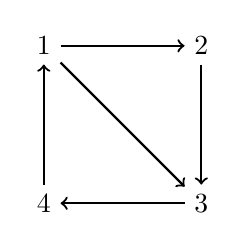
\begin{tikzpicture}
\node (atom1) at (0,2) {1};
\node (atom2) at (2,2) {2};
\node (atom3) at (2,0) {3};
\node (atom4) at (0,0) {4};
\draw[->, thick] (atom1)--(atom2);
\draw[->, thick] (atom2)--(atom3);
\draw[->, thick] (atom3)--(atom4);
\draw[->, thick] (atom4)--(atom1);
\draw[->, thick] (atom1) -- (atom3);
\end{tikzpicture}
\end{center}
Este diagrama é adequado para caracterizar uma interpretação cujo domínio são os números de $1$ a $4$ e que tem uma única relação binária `$\atom{R}{x,y}$', que é verdadeira dos seguintes pares:
	\begin{center}
		\ntuple{1, 2}, 
		\ntuple{2, 3}, 
		\ntuple{3, 4}, 
		\ntuple{4, 1}, 
		\ntuple{1, 3}
	\end{center}
Da mesma forma, podemos oferecer:

\begin{center}
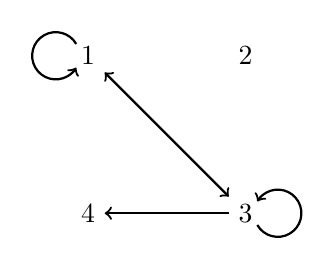
\begin{tikzpicture}
\node (atom1) at (0,2) {1};
\node (atom2) at (2,2) {2};
\node (atom3) at (2,0) {3};
\node (atom4) at (0,0) {4};
\draw[->, thick] (atom3)--(atom4);
\draw[->, thick] (atom1)+(-0.15,0.15) arc (-330:-30:.3); 
\draw[->, thick] (atom3)+(0.15,-0.15) arc (-150:150:.3); 
\draw[<->, thick] (atom1) -- (atom3);
\end{tikzpicture}
\end{center}
para uma interpretação com o mesmo domínio, e com uma relação binária `$\atom{R}{x,y}$' cuja extensão é dada pelos seguintes pares:
	\begin{center}
		\ntuple{1, 3}, 
		\ntuple{3, 1}, 
		\ntuple{3, 4}, 
		\ntuple{1, 1},
		\ntuple{3, 3}
	\end{center}
Se quisermos, podemos tornar nossos diagramas mais complexos. Por exemplo, podemos adicionar nomes como rótulos para objetos específicos.
Da mesma forma, para simbolizar a extensão de um predicado de um lugar, podemos simplesmente desenhar um anel em torno de alguns objetos específicos e estipular que os objetos assim circundados (e somente eles) satisfazem o predicado em questão. 


\chapter{A verdade na LPO}\label{s:TruthFOL}
Não custa nada relembrar aqui que o objetivo principal do estudo da lógica é avaliar argumentos, separando os válidos dos inválidos.
E também não custa nada relembrar que um argumento é válido quando suas premissas justificam sua conclusão, ou seja, quando não é possível haver uma situação em que suas premissas sejam todas verdadeiras, mas sua conclusão seja falsa.
Então, antes de sermos capazes de avaliar argumentos na LPO, precisamos ser capazes de ligar as sentenças da LPO a situações em que poderemos avaliar se elas são verdadeiras ou falsas.

%Na LVF, esta ponte entre as sentenças simbolizadas e as situações é feita pelas valorações.
Na LVF, esta ponte que nos possibilita interpretar sentenças simbolizadas em situações nas quais elas serão verdadeiras ou falsas é dada pelas chaves de simbolização, juntamente com as valorações.
%Através de uma chave de simbolização, situações distintas produzem valorações distintas nas quais as sentenças são verdadeiras ou falsas;
Através de uma chave de simbolização, a verdade ou falsidade das sentenças em português nas diversas situações transforma-se na verdade ou falsidade das sentenças simbolizadas na LVF nas diversas valorações.
Uma chave de simbolização liga situações distintas a valorações distintas que correspondem às diversas linhas das tabelas de verdade, nas quais as sentenças da LVF são verdadeiras ou falsas.
E a consideração dos valores de verdade das sentenças em todas as valorações possíveis, feita nas tabelas de verdade, nos possibilita avaliar a validade dos argumentos.\footnote{
	Se quiser relembrar os detalhes deste processo na LVF, releia a Seção~\ref{s:SustentValid}, p.\,\pageref{s:SustentValid}.}
%e a consideração, através das tabelas de verdade, de todas as valorações possíveis, nos possibilita avaliar a validade dos argumentos.

No caso da LPO, esta ponte entre as sentenças simbolizadas e as situações é feita pela noção de interpretação, introduzida na Seção \ref{s:Interpret}, p.\,\pageref{s:Interpret}.
Vimos ali que uma interpretação é uma chave de simbolização composta por: 
\begin{ebullet}
	\item um domínio do discurso;
	\item uma atribuição (direta ou indireta) de valores de verdade para cada letra sentencial;
	\item a definição de uma referência, no domínio, para cada nome;
	\item a definição (direta ou indireta) de uma extensão para cada predicado e relação.
\end{ebullet}
Uma chave de simbolização com todos esses componentes constitui uma interpretação e nos fornece tudo o que precisamos para decidir se uma sentença qualquer da LPO é verdadeira ou falsa.
Entender como utilizar interpretações para classificar as sentenças da LPO como verdadeiras ou falsas é o primeiro passo para conseguirmos avaliar argumentos na LPO, e será nossa tarefa neste capítulo.

Sabemos, do Capítulo \ref{s:FOLSentences}, que existem três tipos de sentenças na LPO:
	\begin{itemize}
		\item sentenças atômicas:
		\begin{ebullet}
			\item $\atom{C}{b}$
			\item $\atom{A}{r,j}$
			\item $Q$
		\end{ebullet}
		\item sentenças cujo operador principal é um conectivo sentencial:
		\begin{ebullet}
			\item $\atom{C}{b} \eand Q$
			\item $\atom{A}{r,j} \eif \forall x\,\atom{C}{x}$
			\item $\enot Q$
		\end{ebullet}
		\item sentenças cujo operador principal é um quantificador:
		\begin{ebullet}
			\item $\exists x\,\atom{C}{x}$
			\item $\forall x (\atom{A}{x,j} \eif \atom{C}{x})$
			\item $\exists x \exists y (\atom{A}{x,y} \eand \atom{A}{y,x})$
		\end{ebullet}
	\end{itemize}
Temos que explicar como atribuir valores de verdade para cada um destes tipos de sentenças.

A explicação que daremos aqui é completamente geral e vale para qualquer interpretação.
No entanto, para facilitar a compreensão, usaremos a seguinte interpretação como exemplo privilegiado:
\begin{center}\label{i:Sample}
	\begin{ekey}
		\item[\text{domínio}] {\small todas as pessoas (vivas ou mortas) nascidas antes do ano 2020}
		\item[a] {\small Aristóteles}
		\item[b] {\small Simona Talma}
		\item[C] {\small Simona Talma é uma artista potiguar\,}\footnote{
			Poderíamos aqui ter criado um predicado tal como `$\atom{P}{x}$' para `\gap{x}~é uma artista portiguar' e simbolizar `Simona Talma é uma artista potiguar' como `$\atom{P}{b}$'.
			Não fizemos isso porque queremos que a interpretação de nosso exemplo tenha também uma letra sentencial `$C$' que, tal  como na LVF, tem exatamente o mesmo valor de verdade que a sentença `Simona Talma é uma artista potiguar'.}
		\item[D] {\small é F (uma sentença falsa)}\footnote{
			Aqui estamos apenas indicando diretamente, sem nenhuma sentença em português intermediária, que a letra sentencial `$D$' é uma sentença falsa.}
		\item[\atom{F}{x}] \gap{x} {\small é filósofo}
		\item[\atom{R}{x,y}] \gap{x} {\small nasceu antes que} \gap{y}
	\end{ekey}
\end{center}
Esta interpretação será o nosso caso de estudo nas Seções seguintes.


\section{Sentenças atômicas}
Existem três tipos de sentenças atômicas na LPO, as letras sentenciais, tais como `$C$' e `$D$', os predicados seguidos de nomes, tais como  `$\atom{F}{a}$' e `$\atom{F}{b}$', e as relações $n$-árias seguidas de $n$-uplas ordenadas de nomes, tais como `$\atom{R}{a,b}$' e `$\atom{R}{b,a}$'.
Precisamos, então, entender como as interpretações atribuem valores de verdade para cada um desses três tipos de sentenças atômicas.

No caso das letras sentenciais, isso é uma operação imediata idêntica ao que fazíamos na LVF.
A interpretação estabelece direta ou indiretamente se a letra sentencial é verdadeira ou falsa.
Em nosso exemplo
\begin{center}
	$`C'$ \ \ é \ \ verdadeira   
\end{center}
porque Simona Talma é mesmo uma artista potiguar.
A interpretação nos dá aqui uma especificação indireta através da sentença em português `Simona Talma é uma artista potiguar'.
A letra sentencial terá o mesmo valor de verdade desta sentença.

Por outro lado,
\begin{center}
	$`D'$ \ \ é \ \ falsa   
\end{center}
porque a interpretação estabelece diretamente este fato, sem qualquer sentença intermediária.

%Se a sentença atômica for constituída por um predicado seguido de um nome, tal como `$\atom{F}{a}$', ela será verdadeira apenas no caso do predicado `$\atom{F}{x}$' ser verdadeiro do indivíduo que `$a$' nomeia.
Quando a sentença atômica é constituída por um predicado seguido de um nome, tal como `$\atom{F}{a}$', ela será verdadeira apenas no caso em que o indivíduo que `$a$' nomeia esteja na extensão do predicado `$\atom{F}{x}$'.
Em nossa interpretação, a extensão de `$\atom{F}{x}$' é dada indiretamente pelo predicado `\gap{x} é filósofo'.
Então,
\begin{center}
	`$\atom{F}{a}$' \ \ é \ \ verdadeira
\end{center}
já que `$a$' nomeia Aristóteles e Aristóteles é um filósofo.
De modo semelhante,
\begin{center}
	`$\atom{F}{b}$' \ \ é \ \ falsa
\end{center}
porque `$b$' nomeia Simona Talma, que não é uma filósofa.

Por fim, se a sentença atômica for uma relação seguida de uma sequência ordenada de nomes, tal como `$\atom{R}{a,b}$', ela será verdadeira apenas se o par ordenado dos indivíduos nomeados por `$a$' e `$b$', \ntuple{Aristóteles, Simona Talma}, estiver na extensão do predicado `$\atom{R}{x,y}$'.
Em nossa interpretação esta extensão é definida indiretamente através da relação
\begin{center}
	`\gap{x} nasceu antes que \gap{y}'.
\end{center}	
Como Aristóteles nasceu antes de Simona Talma, então o par \ntuple{Aristóteles, Simona Talma} está na extensão de `$\atom{R}{x,y}$' e
\begin{center}
	`$\atom{R}{a,b}$' \ \ é \ \ verdadeira
\end{center}
Da mesma forma, podemos facilmente verificar que 
\begin{center}
	`$\atom{R}{a,a}$' \ \ é \ \ falsa
\end{center}
porque Aristóteles não nasceu antes que Aristóteles.

Lidar com sentenças atômicas é, portanto, muito intuitivo.
As letras sentencias são tratadas exatamente do mesmo modo que na LVF e quando \meta{R} é um predicado $n$-lugares e \mbox{$\meta{a}_1 $, $\meta{a}_{2}$, \dots, $\meta{a}_{n}$} \ são nomes, temos:

	\factoidbox{
		$\atom{\meta{R}}{\meta{a}_{1},\meta{a}_{2},\dots,\meta{a}_{n}}$ é verdadeira em uma interpretação\\
		\textbf{se e somente se}\\
		$\meta{R}$ é verdadeira dos objetos nomeados por $\meta{a}_{1}$, $\meta{a}_{2}$, \dots, $\meta{a}_{n}$ na interpretação (considerados nesta ordem)
	}
Lembre-se, porém, de que existe um tipo especial de sentença atômica: dois nomes conectados por um sinal de identidade constituem uma sentença atômica.
Esse tipo de sentença atômica também é fácil de lidar.
Sejam \meta{a} e \meta{b} nomes quaisquer,
	\factoidbox{
		$\meta{a} = \meta{b}$ é verdadeira em uma interpretação\\
		\textbf{se e somente se}\\
		 \meta{a} e \meta{b} são nomes do mesmo objeto nesta interpretação
	}
Portanto, em nossa interpretação,
\begin{center}
	`$a=b$' \ \ é \ \ falsa
\end{center}
porque Aristóteles e Simona Talma não são a mesma pessoa.


\section{Conectivos sentenciais}
Vimos no Capítulo \ref{s:FOLSentences} que as sentenças da LPO podem ser criadas a partir de sentenças mais simples, usando os conectivos verofuncionais da LVF. As regras que governam a atribuição de verdade ou falsidade a sentenças deste tipo na LPO são \emph{exatamente} as mesmas da LVF.
Aqui estão elas:
	\factoidbox{
		$\meta{A} \eand \meta{B}$ é verdadeira em uma interpretação\\ \textbf{se e somente se}\\
		$\meta{A}$ e $\meta{B}$ são ambas verdadeiras nesta interpretação
		
		\bigskip
		$\meta{A} \eor \meta{B}$ é verdadeira em uma interpretação\\  \textbf{se e somente se}\\
		$\meta{A}$ é verdadeira ou $\meta{B}$ é verdadeira nesta interpretação

		\bigskip
		$\enot \meta{A}$ é verdadeira em uma interpretação\\ \textbf{se e somente se}\\
		$\meta{A}$ é falsa nesta interpretação

		\bigskip
		$\meta{A} \eif \meta{B}$ é verdadeira em uma interpretação\\ \textbf{se e somente se}\\
		$\meta{A}$ é falsa ou $\meta{B}$ é verdadeira nesta interpretação

		\bigskip
		$\meta{A} \eiff \meta{B}$ é verdadeira em uma interpretação\\ \textbf{se e somente se}\\
		$\meta{A}$ e $\meta{B}$ têm o mesmo valor de verdade nesta interpretação
	}\label{b:ConSent}
Estas definições nos dão, de um modo diferente, exatamente a mesma informação que as tabelas de verdade características dos conectivos, que vimos no Capítulo \ref{s:CharacteristicTruthTables}, p.\,\pageref{s:CharacteristicTruthTables}.
Alguns exemplos nos ajudarão aqui.
A ideia é aplicar as definições do quadro acima à nossa interpretação exemplo (p.\,\pageref{i:Sample}) para decidir o valor de verdade das sentenças:
	\begin{earg}
		\item[\textbullet] `$a = a \eand \atom{F}{a}$' \ \ é \ \ verdadeira\\
			porque tanto `$a = a$' quanto `$\atom{F}{a}$' são verdadeiras\\
		\item[\textbullet] `$\atom{R}{a,b} \eand \atom{F}{b}$' \ \ é \ \ falsa\\
			porque ainda que `$\atom{R}{a,b}$' seja verdadeira, `$\atom{F}{b}$' é falsa\\
		\item[\textbullet] `$a = b \eor \atom{F}{a}$' \ \ é \ \ verdadeira\\
			porque ainda que  `$a = b$' seja falsa, `$\atom{F}{a}$' é verdadeira\\
		\item[\textbullet] `$\enot a = b$' \ \ é \ \ verdadeira\\
			porque `$a = b$' é falsa\\
		\item[\textbullet] `$\atom{F}{a} \eand \enot( a= b \eand \atom{R}{a,b})$' \ \ é \ \ verdadeira\\
			porque `$\atom{F}{a}$' é verdadeira e `$a = b$' é falsa
	\end{earg}
Antes de prosseguir, certifique-se de ter compreendido todos esses exemplos.
Simplesmente aplicamos, em cada caso, a definição correspondente do quadro acima (p.\,\pageref{b:ConSent}). 


\section[Quantificadores]{Quando o operador principal é um quantificador}\label{s:MainLogicalOperatorQuantifier}
Até aqui viemos bem, mas ainda não tratamos do aspecto que representa a principal novidade introduzida na LPO:
as sentenças cujo operador principal é um \emph{quantificador}.
Veremos que expressar as condições de verdade deste tipo de sentenças é um pouco mais complicado do que parece à primeira vista.
A ideia geral até que é simples e já foi mencionada de passagem em capítulos anteriores:
	\begin{earg}
		\item[\textbullet] $\forall x \atom{\meta{A}}{x}$ é verdadeira \ \ \textbf{se e somente se}\\
		$\atom{\meta{A}}{x}$ for verdadeira \textit{de todos} os elementos do domínio.\\
		\item[\textbullet] $\exists x \atom{\meta{B}}{x}$ é verdadeira \ \ \textbf{se e somente se}\\
		$\atom{\meta{B}}{x}$ for verdadeira \textit{de algum} elemento do domínio.
	\end{earg}
A dificuldade maior não é esta ideia geral, mas a especificação de sua definição precisa.

Vamos aqui nos aproximar pouco a pouco da definição.
Começaremos com algumas propostas ingênuas e vamos corrigindo-as até, eventualmente, chegarmos à definição correta.
Uma primeira proposta é a seguinte:
se, como vimos, `$\forall x\,\atom{F}{x}$' deve ser verdadeira se e somente se `$\atom{F}{x}$' é verdadeira para tudo no domínio,
então poderíamos simplesmente considerar que uma sentença universal é verdadeira quando a extensão do predicado que a segue compreende todo o domínio do discurso.

Esta ideia funciona quando o que vem após o quantificador inicial é um predicado, como em  `$\forall x\,\atom{F}{x}$'.
Mas, infelizmente, essa ideia não é geral o suficiente para especificar as condições de verdade de sentenças onde o que segue o quantificador inicial não é um predicado, mas outra expressão quantificada, tal como ocorre em:
$$\forall x \exists y\,\atom{L}{x,y}$$
Não conseguimos aplicar esta ideia aqui, porque o que segue o quantificador não é um predicado, mas a expressão quantificada `$\exists y\,\atom{L}{x,y}$'.
E as interpretações não têm cláusulas que indicam se `$\exists y\,\atom{L}{x,y}$' é verdadeira de tudo no domínio.
As cláusulas das intepretações especificam apenas a referência de nomes e a extensão de predicados e relações.

Para tentar corrigir isso poderíamos então sugerir que `$\forall x \exists y\, \atom{L}{x,y}$' deve ser verdadeira em uma interpretação se e somente se $\exists y\, \atom{L}{\meta{a},y}$ for verdadeira para \emph{todo} nome \meta{a} da interpretação.
E, de modo similar, diríamos que $\exists y\, \atom{L}{\meta{a},y}$ é verdadeira se e somente se $\atom{L}{\meta{a}, \meta{b}}$ for verdadeira para \emph{algum} nome \meta{b}.
Então, juntando estes dois passos, `$\forall x \exists y\, \atom{L}{x,y}$' seria verdadeira em uma interpretação se e somente se $\atom{L}{\meta{a}, \meta{b}}$ for verdadeira para \emph{todo} nome \meta{a} e \emph{algum} nome \meta{b} presentes na interpretação.

Infelizmente, isso também não funciona.
Para entender por que, basta observar que na interpretação de nossos exemplos (p.\,\pageref{i:Sample}), apenas duas pessoas têm nome, mas o domínio comporta todas as pessoas nascidas antes do ano 2020.

Uma terceira ideia, então, é a seguinte.
Mesmo que uma interpretação não tenha nomes para \emph{todos} os indivíduos do domínio, ela poderia ter.
Ou seja, podemos estender uma interpretação qualquer, de modo a que todos os elementos do domínio tenham nomes.
Antes de prosseguir com a definição, vejamos alguns exemplos de como isso pode funcionar.

Em nossa interpretação privilegiada (p.\,\pageref{i:Sample}) `$\exists x\, \atom{R}{b,x}$' deve ser verdadeira. Afinal, certamente há no domínio alguém que nasceu depois que Simona Talma.
Dani Cruz (uma outra artista potiguar) é uma dessas pessoas.
De fato, se estendermos temporariamente nossa interpretação adicionando o nome `$c$' para se referir a Dani Cruz, então `$\atom{R}{b,c}$' será verdadeira nessa interpretação estendida.
E este fato certamente deve ser suficiente para assegurar que `$\exists x\,\atom{R}{b,x}$' é verdadeira na nossa interpretação original, já que ele indica que há pelo menos uma pessoa no domínio (Dani Cruz) que nasceu depois de Simona Talma.

Na nossa interpretação, `$\exists x (\atom{F}{x} \eand \atom{R}{x,a})$' também deve ser verdadeira.
Afinal, no domínio, certamente há alguém que foi filósofo e nasceu antes de Aristóteles.
Sócrates é uma dessas pessoas.
De fato, se estendermos nossa interpretação, com um novo nome, `$d$', que denota Sócrates, então `$\atom{F}{d} \eand \atom{R}{d,a}$' será verdadeira nessa interpretação estendida.
Novamente, isso certamente é suficiente como garantia de que `$\exists x (\atom{F}{x} \eand \atom{R}{x,a})$' é verdadeira na interpretação original (não estendida), já que isso indica que há pelo menos uma pessoa no domínio (Sócrates) que é filósofo e nasceu antes de Aristóteles.

Já a sentença `$\forall x \exists y\, \atom{R}{x,y}$' deve ser falsa em nossa interpretação.
Afinal, certamente há uma última pessoa que nasceu antes do ano 2020 começar.
Não sabemos quem é esta pessoa, mas podemos, mesmo assim, estender a interpretação para que um nome novo, `$e$', denote exatamente esta pessoa.
E fazendo isso, qualquer que seja o indivíduo do domínio ao qual um outro nome novo $`f'$ se refira, a sentença `$\atom{R}{e,f}$' seria falsa.
De fato, não importa \emph{quem} seja a referência do nome `$f$', sabemos que `$\atom{R}{e,f}$' será falsa, já que `$e$' denota a última pessoa nascida em 2019. 
Esse fato é certamente suficiente para garantir que `$\exists y\, \atom{R}{e,y}$' é falsa na interpretação estendida. E isso, por sua vez, é certamente suficiente como garantia de que `$\forall x \exists y\, \atom{R}{x,y}$' é falsa na nossa interpretação original.

Se você entendeu esses três exemplos, ótimo. É isso que importa.
O que temos que fazer, agora, é fornecer uma definição precisa dessas ideias, que exprima as condições de verdade para sentenças quantificadas.
Para isso precisamos de mais notação em nossa metalinguagem.
A expressão:
$$\meta{A}(\meta{x})$$
será usada para denotar na metalinguagem uma fórmula que contenha pelo menos uma ocorrência livre da variável \meta{x}.
Ou seja, há uma ou mais ocorrências de \meta{x} em \meta{A} que estão fora do escopo de qualquer `$\forall x$' e `$\exists x$' em \meta{A}.
Seja \meta{c} um nome.
A expressão:
$$\meta{A}(\meta{c})$$
será usada para denotar na metalinguagem a fórmula obtida quando substituímos por $\meta{c}$ \emph{todas} as ocorrências livres de $\meta{x}$ em \meta{A}.
A fórmula resultante, $\meta{A}(\meta{c})$, é chamada de \define{substitution instance} de $\forall \meta{x} \meta{A}$ e $\exists \meta{x} \meta{A}$.
Além disso, $\meta{c}$ é chamado de nome de instanciação.

Vejamos um exemplo.
Considere a sentença da LPO:
	$$\forall y \exists x (\atom{R}{y,x} \eiff \atom{F}{x})$$
A notação recém  introduzida nos permite usar a expressão
	$$\forall \meta{y} \atom{\meta{A}}{\meta{y}}$$
para nos referirmos a esta sentença de um modo genérico em nossa metalinguagem.
Quando fazemos isso, a expressão
	$$\atom{\meta{A}}{\meta{y}}$$
refere-se genericamente a
	$$\exists x (\atom{R}{y,x} \eiff \atom{F}{x})$$
que é uma fórmula com uma ocorrência livre da variável `$y$'.
Se substituímos esta ocorrência livre de `$y$' por um nome, digamos, `$e$', obtemos a sentença:
	$$\exists x (\atom{R}{e,x} \eiff \atom{F}{x})$$
Esta sentença nada mais é do que uma instância de substituição de 
	$$\forall y \exists x (\atom{R}{y,x} \eiff \atom{F}{x})$$
onde `$e$' é o nome de instanciação, e `$y$' é a variável instanciada.

Seja $\mathbf{I}$ o nome de uma interpretação que estejamos considerando.
$\mathbf{I}$ inclui uma especificação de quais nomes correspondem a quais objetos no domínio.
Considere um objeto  qualquer do domínio, digamos, $d$, e um nome $\meta{c}$ que não esteja sendo usado em $\mathbf{I}$.
Usaremos a notação
$$\mathbf{I}[d/\meta{c}]$$
para nos referirmos à interpretação que é igual a $\mathbf{I}$, com um acréscimo:
$\mathbf{I}[d/\meta{c}]$ atribui o nome $\meta{c}$ ao objeto $d$.
Então podemos dizer que $d$ \define{satisfacao} a fórmula $\meta{A}(\meta{x})$ na interpretação $\mathbf{I}$ se e somente se $\meta{A}(\meta{c})$ é verdadeira em $\mathbf{I}[d/\meta{c}]$.
(Quando $d$ satisfaz $\meta{A}(\meta{x})$, nós dizemos também que $\meta{A}(\meta{x})$ é \emph{verdadeira de} $d$.

\factoidbox{A interpretação $\mathbf{I}[d/\meta{c}]$ é igual à interpretação $\mathbf{I}$, com o acréscimo de que atribui o nome $\meta{c}$ ao objeto $d$.

\
\\
Um objeto $d$ \define{satisfacao} $\meta{A}(\meta{x})$ na interpretação $\mathbf{I}$ \\
\hbox{\textbf{se e somente se}} $\meta{A}(\meta{c})$ é verdadeira em $\mathbf{I}[d/\meta{c}]$.
}

\noindent Assim, por exemplo, dizemos que: 
\begin{ebullet}
	\item Sócrates \underline{satisfaz} a fórmula `$\atom{F}{x}$'
\end{ebullet}
pois:
\begin{ebullet}
	\item $\atom{F}{c}$ é \underline{verdadeira} na interpretação $\mathbf{I}[\text{Sócrates}/c]$
\end{ebullet}
ou seja, $\atom{F}{c}$ é verdadeira na interpretação que obtemos de nossa interpretação original $\mathbf{I}$ (p.\pageref{i:Sample}) quando acrescentamos a indicação de que o nome `$c$' se refere a Sócrates:

\begin{center}
	\begin{ekey}
		\item[\text{domínio}] {\small todas as pessoas (vivas ou mortas) nascidas antes do ano 2020}
		\item[a] {\small Aristóteles}
		\item[b] {\small Simona Talma}
		\item[c] {\small Sócrates}
		\item[C] {\small Simona Talma é uma artista potiguar\,}
		\item[D] {\small é F (uma sentença falsa)}
		\item[\atom{F}{x}] \gap{x} {\small é filósofo}
		\item[\atom{R}{x,y}] \gap{x} {\small nasceu antes que} \gap{y}
	\end{ekey}
\end{center}

Tendo ampliado nossa metalinguagem com estas notações, podemos finalmente definir as condições de verdade de sentenças da LPO cujo operador principal é um quantificador.
A ideia aproximada é a seguinte.
A sentença $\forall \meta{x}\meta{A}(\meta{x})$ será verdadeira em $\mathbf{I}$ se e somente se, para qualquer objeto $d$ no domínio, $\meta{A}(\meta{c})$ é verdadeira em $\mathbf{I}[d/\meta{c}]$.
Ou seja, $\forall \meta{x}\meta{A}(\meta{x})$ será verdadeira  se e somente se $\meta{A}(\meta{c})$ for verdadeira, independentemente de qual objeto (no domínio) tenha sido nomeado  por $\meta{c}$.
Em outras palavras, $\forall \meta{x} \meta{A}(\meta{x})$ é verdadeira apenas quando todos os objetos no domínio satisfazem $\meta{A}(\meta{x})$.

Similarmente, a sentença $\exists \meta{x}\meta{A}(\meta{x})$ será verdadeira se e somente se houver \emph{algum} objeto no domínio que satisfaça $\meta{A}(\meta{x})$.
Ou seja, $\exists \meta{x}\meta{A}(\meta{x})$ é verdadeira em $\mathbf{I}$ se e somente se  $\meta{A}(\meta{c})$ é verdadeira em $\mathbf{I}[d/\meta{c}]$ para pelo menos um objeto $d$.
	\factoidbox{
		$\forall \meta{x}\meta{A}(\meta{x})$ é \underline{verdadeira} em uma interpretação \textbf{se e somente se} todo objeto no domínio \underline{satisfiaz} $\meta{A}(\meta{x})$.
		
		\
		\\
		$\exists \meta{x}\meta{A}(\meta{x})$ é \underline{verdadeira} em uma interpretação \textbf{se e somente se} pelo menos um objeto no domínio \underline{satisfaz} $\meta{A}(\meta{x})$.
	}
Para ficar claro: tudo o que estamos fazendo aqui é formalizar (de um modo bastante preciso) a ideia intuitiva de que para que uma sentença quantifidada universalmente seja verdadeira, todos os objetos do domínio precisam satisfazê-la; e para que uma sentença quantificada existencialmente seja verdadeira, basta que um objeto do domínio a satisfaça. 

Finalmente, vale notar que o conceito de um objeto satisfazer uma fórmula com uma variável livre também pode ser estendido a fórmulas com mais de uma variável livre.
Por exemplo, se tivermos uma fórmula $\meta{A}(\meta{x},\meta{y})$ com duas variáveis livres $\meta{x}$ e $\meta{y}$, podemos dizer que um par de objetos $\langle a, b\rangle$ satisfaz $\meta{A}(\meta{x},\meta{y})$ se e somente se $\meta{A}(\meta{c},\meta{d})$ for verdadeira na interpretação estendida por dois nomes $\meta{c}$ e $\meta{d}$, onde $\meta{c}$ é o nome de $a$ e $\meta{d}$ é o nome de $b$.
Assim, por exemplo, $\langle \text{Sócrates}, \text{Platão}\rangle$ satisfaz $R(x,y)$, pois, já que Sócrates nasceu antes de Platão, $R(c,d)$ é verdadeiro na interpretação:
\begin{center}
	\begin{ekey}
		\item[\text{domínio}] {\footnotesize todas as pessoas (vivas ou mortas) nascidas antes do ano 2020}
		\item[a] {\small Aristóteles}
		\item[b] {\small Simona Talma}
		\item[c] {\small Sócrates}
		\item[d] {\small Platão}
		\item[C] {\small Simona Talma é uma artista potiguar\,}
		\item[D] {\small é F (uma sentença falsa)}
		\item[\atom{F}{x}] \gap{x} {\small é filósofo}
		\item[\atom{R}{x,y}] \gap{x} {\small nasceu antes que} \gap{y}
	\end{ekey}
\end{center}
Para fórmulas atômicas, tais como $\atom{F}{x}$ e $\atom{R}{x,y}$,  os objetos ou sequências de objetos que as satisfazem são exatamente a extensão dos predicados que as constituem.
Mas a noção de satisfação também se aplica a fórmulas não atômicas.
A fórmula $\atom{F}{x} \land \atom{R}{x,b}$, por exemplo, é satisfeita por todos os filósofos que nasceram antes de Simona Talma.
A ideia de satisfação aplica-se até mesmo a fórmulas envolvendo quantificadores.
Por exemplo, $F(x) \eand \lnot\exists y(F(y) \land R(y,x))$ é satisfeita por todos os filósofos para os quais nenhum filósofo nasceu antes deles---em outras palavras, o primeiro filósofo, e apenas ele, satisfaz esta fórmula.


\practiceproblems
\solutions
\problempart
\label{pr.TorF1}
Considere a seguinte interpretação:
	\begin{ebullet}\small
		\item O domínio compreende apenas Benedita e Clayton
		\item `$\atom{A}{x}$' é verdadeira para ambos, tanto Benedita quanto Clayton
		\item `$\atom{B}{x}$' é verdadeira apenas para Benedita
		\item `$\atom{N}{x}$' não é verdadeira nem para Benedita nem para Clayton
		\item `$c$' refere-se a Clayton
	\end{ebullet}
Para cada uma das nove sentenças seguintes, determine se ela é verdadeira ou falsa nesta interpretação.
\begin{earg}
\item $\atom{B}{c} $
\item $\atom{A}{c}  \eiff \enot \atom{N}{c}$
\item $\atom{N}{c}  \eif (\atom{A}{c} \eor \atom{B}{c})$
\item $\forall x\, \atom{A}{x}$
\item $\forall x \enot \atom{B}{x}$
\item $\exists x(\atom{A}{x} \eand \atom{B}{x})$
\item $\exists x(\atom{A}{x} \eif \atom{N}{x})$
\item $\forall x(\atom{N}{x} \eor \enot \atom{N}{x})$
\item $\exists x\, \atom{B}{x} \eif \forall x\, \atom{A}{x}$
\end{earg}

\problempart
\label{pr.TorF2}
Considere a seguinte interpretação:	
	\begin{ebullet}
		\item O domínio compreende apenas Leila, Cora e Ênio
		\item `$\atom{G}{x}$' é verdadeira de Leila, de Cora e de Ênio
		\item `$\atom{H}{x}$' é verdadeira apenas de Cora
		\item `$\atom{M}{x}$' é verdadeira apenas de Leila e Ênio
		\item `$c$' refere-se a Cora
		\item `$e$' refere-se a Ênio
	\end{ebullet}
Para cada uma das quinze sentenças seguintes, determine se ela é verdadeira ou falsa nesta interpretação.
\begin{earg}
\item $\atom{H}{c} $
\item $\atom{H}{e} $
\item $\atom{M}{c}  \eor \atom{M}{e}$
\item $\atom{G}{c}  \eor \enot \atom{G}{c}$
\item $\atom{M}{c}  \eif \atom{G}{c}$
\item $\exists x\, \atom{H}{x}$
\item $\forall x\, \atom{H}{x}$
\item $\exists x\, \enot \atom{M}{x}$
\item $\exists x(\atom{H}{x} \eand \atom{G}{x})$
\item $\exists x(\atom{M}{x} \eand \atom{G}{x})$
\item $\forall x(\atom{H}{x} \eor \atom{M}{x})$
\item $\exists x\, \atom{H}{x} \eand \exists x\, \atom{M}{x}$
\item $\forall x(\atom{H}{x} \eiff \enot \atom{M}{x})$
\item $\exists x\, \atom{G}{x} \eand \exists x \enot \atom{G}{x}$
\item $\forall x\exists y(\atom{G}{x} \eand \atom{H}{y})$
\end{earg}

\problempart
\label{pr.TorF3}
Conforme as convenções introduzidas no final do Capítulo~\ref{s:Interpretations} (p.\,\pageref{s:Interpret}), o diagrama abaixo especifica uma interpretação cujo domínio é o conjunto $\{1,2,3,4,5\}$ e que tem uma única relação binária $\atom{R}{x,y}$, cuja extensão é dada pelas setas do diagrama:
\begin{center}
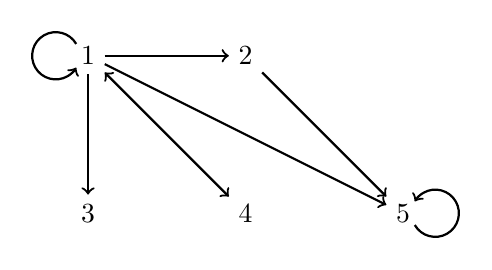
\begin{tikzpicture}
\node (atom1) at (0,2) {1};
\node (atom2) at (2,2) {2};
\node (atom4) at (0,0) {3};
\node (atom5) at (2,0) {4};
\node (atom6) at (4,0) {5};
\draw[->, thick] (atom1)+(-0.15,0.15) arc (-330:-30:.3); 
\draw[->, thick] (atom6)+(0.15,-0.15) arc (-150:150:.3); 
\draw[->, thick] (atom1) -- (atom2);
\draw[->, thick] (atom1) -- (atom4);
\draw[<->, thick] (atom1) -- (atom5);
\draw[->, thick] (atom1) -- (atom6);
\draw[->, thick] (atom2) -- (atom6);
\end{tikzpicture}
\end{center}
Para cada uma das doze sentenças seguintes, determine se ela é verdadeira ou falsa nesta interpretação.
\begin{earg}
\item $\exists x\, \atom{R}{x,x}$
\item $\forall x\, \atom{R}{x,x}$
\item $\exists x \forall y\, \atom{R}{x,y}$
\item $\exists x \forall y\, \atom{R}{y,x}$
\item $\forall x \forall y \forall z ((\atom{R}{x,y} \eand \atom{R}{y,z}) \eif \atom{R}{x,z})$
\item $\forall x \forall y \forall z ((\atom{R}{x,y} \eand \atom{R}{x,z}) \eif \atom{R}{y,z})$
\item $\exists x \forall y\, \enot \atom{R}{x,y}$
\item $\forall x(\exists y\, \atom{R}{x,y} \eif \exists y\, \atom{R}{y,x})$
\item $\exists x \exists y (\enot x = y \eand \atom{R}{x,y} \eand \atom{R}{y,x})$
\item $\exists x \forall y(\atom{R}{x,y} \eiff x = y)$
\item $\exists x \forall y(\atom{R}{y,x} \eiff x = y)$
\item $\exists x \exists y(\enot x = y \eand \atom{R}{x,y} \eand \forall z(\atom{R}{z,x} \eiff y = z))$
\end{earg}


\chapter{Conceitos semânticos}

Oferecer uma definição precisa de sentença verdadeira na LPO foi um pouco complicado, mas agora que terminamos, podemos definir várias noções lógicas importantes.
Elas serão muito parecidas com as definições que oferecemos para a LVF.
No entanto, lembre-se de que agora elas se referem a \emph{interpretações}, e não mais a valorações.

Continuaremos a usar o símbolo `$\entails$' na LPO da mesma forma que o utilizamos na LVF.
Assim:
	$$\meta{A}_1, \meta{A}_2, \ldots, \meta{A}_n \entails\meta{C}$$
significa que não há interpretação na qual $\meta{A}_1$, $\meta{A}_2$, \dots, $\meta{A}_n$ sejam todas verdadeiras e \meta{C} seja falsa. Consequentemente,
	$$\entails\meta{A}$$
significa que \meta{A} é verdadeira em todas as interpretações, ou seja, que é impossível que \meta{A} seja falsa.

As outras noções lógicas que vimos, também têm definições correspondentes na LPO.
Aqui estão elas:

\begin{itemize}
\item Uma sentença  $\meta{A}$ é uma \define{validity} se e somente se $\meta{A}$ for verdadeira em todas as interpretações; ou seja, se
$$\entails\meta{A}$$ \label{def:validade_logica}
\item $\meta{A}$ é uma \define{contradiction of FOL} se e somente se $\meta{A}$ for falsa em todas as interpretações; ou seja, se
$$\entails\enot\meta{A}$$
\item $\meta{A}_1, \meta{A}_2, \ldots \meta{A}_n \therefore \meta{C}$ é um argumento \define{valid in FOL} se e somente se não houver interpretação em que todas as premissas são verdadeiras e a conclusão é falsa; ou seja, se
$$\meta{A}_1,\meta{A}_2,\ldots \meta{A}_n \entails\meta{C}$$

\item Um argumento $\meta{A}_1, \meta{A}_2, \ldots \meta{A}_n \therefore \meta{C}$ é \textit{invalido na LPO} se e somente se ele não é válido, ou seja, quando há alguma interpretação na qual todas as suas premissas são verdadeiras e a conclusão é falsa.
Denotamos isso por:
$$\meta{A}_1,\meta{A}_2,\ldots \meta{A}_n \nvDash\meta{C}$$
 
\item Duas sentenças da LPO \meta{A} e \meta{B} são \define{equivalent in FOL} se e somente se em toda interpretação na qual uma é verdadeira, a outra também é; ou seja, se
\begin{center}
	$\meta{A}\entails\meta{B}$ \ \ \ e \ \ \ $\meta{B}\entails\meta{A}$
\end{center}

\item As sentenças $\meta{A}_1$, $\meta{A}_2$, \dots, $\meta{A}_n$ são \define{satisfiable in FOL} se e somente se há alguma interpretação na qual todas são verdadeiras.
Elas são \textit{incompatíveis na LPO} se não houver tal interpretação.
\end{itemize}


\chapter{Utilizando as interpretações}
\label{sec.UsingModels}

\section{Validades e contradições}
Suponha que queremos mostrar que
$$\exists x\, \atom{A}{x,x} \eif \atom{B}{d}$$
\emph{não é} uma validade.
Conforme a definição vista no capítulo anterior, temos que mostrar que esta  sentença não é verdadeira em todas as interpretações; isto é, que ela é falsa em alguma interpretação.
Então será suficiente fornecermos uma única interpretação na qual a sentença seja falsa.

Para que `$\exists x\,\atom{A}{x,x} \eif \atom{B}{d}$' seja falsa, o antecedente do condicional `$\exists x\, \atom{A}{x,x}$' deve ser verdadeiro, e o consequente `$\atom{B}{d}$' deve ser falso.
Para construir uma interpretação na qual isso ocorra, começamos especificando um domínio.
Manter o domínio pequeno facilita a especificação da extensão dos predicados; portanto, começaremos com um domínio com apenas um indivíduo.
Digamos, então, que o único indivíduo de nosso domínio seja a cidade de Fortaleza.
\begin{center}
	\begin{ekey}
		\item[\text{domínio}] Fortaleza
	\end{ekey}
\end{center}
Nossa sentença tem um nome, `$d$', que precisa nomear algo no domínio.
Então nossa única opção é definir que:
\begin{center}
	\begin{ekey}
		\item[d] Fortaleza
	\end{ekey}
\end{center}
Lembre-se de que queremos que `$\exists x\, \atom{A}{x,x}$' seja verdadeira; portanto, queremos que algum indivíduo do domínio relacione-se consigo mesmo através de `$A$'.
Podemos então propor a seguinte extensão para a relação `$A$':
\begin{center}
	\begin{ekey}
		\item[\atom{A}{x,y}] \gap{x} está no mesmo país que \gap{y}
	\end{ekey}
\end{center}
Agora, `$\atom{A}{d,d}$' é claramente verdadeira, portanto, `$\exists x\, \atom{A}{x,x}$' também é. 
Mas nós também queremos que `$\atom{B}{d}$' seja falsa; portanto, o indivíduo nomeado por `$d$' não deve estar na extensão de `$B$'.
Podemos simplesmente propor que:
\begin{center}
	\begin{ekey}
		\item[\atom{B}{x}] \gap{x} é a capital do Rio Grande do Norte
	\end{ekey}
\end{center}
Construímos uma interpretação em que `$\exists x\, \atom{A}{x,x}$' é verdadeira, mas `$\atom{B}{d}$' é falsa.
Logo, nesta interpretação `$\exists x\, \atom{A}{x,x} \eif \atom{B}{d}$' é falsa e portanto não é uma validade.

Com a mesma facilidade podemos mostrar que `$\exists x\atom{A}{x,x} \eif \atom{B}{d}$' não é uma contradição.
Precisamos apenas especificar uma interpretação na qual `$\exists x\atom{A}{x,x} \eif \atom{B}{d}$' seja verdadeira; ou seja, uma interpretação na qual `$\exists x\, \atom{A}{x,x}$' é falsa ou `$\atom{B}{d}$' é verdadeira.
Aqui está uma:
\begin{center}
	\begin{ekey}
		\item[\text{domínio}] Fortaleza
		\item[d] Fortaleza
		\item[\atom{A}{x,y}] \gap{x} está no mesmo país que \gap{y}
		\item[\atom{B}{x}] \gap{x} é a capital do Ceará
	\end{ekey}
\end{center}
Isso mostra que existe uma interpretação na qual `$\exists x\atom{A}{x,x} \eif \atom{B}{d}$' é verdadeira, e portanto, não é uma contradição.
	\factoidbox{
		Para mostrar que $\meta{A}$ \textbf{não é uma validade}, basta apresentar uma interpretação em que $\meta{A}$ seja falsa.\\
		
		Para mostrar que $\meta{A}$ \textbf{não é uma contradição}, basta apresentar uma interpretação em que $\meta{A}$ seja verdadeira.
	}


\section{Equivalência lógica}
Suponha que queiramos mostrar que
\begin{center}
	$\forall x\, \atom{S}{x}$ \ \ e \ \ $\exists x\, \atom{S}{x}$
\end{center}
\emph{não são} logicamente equivalentes.
Precisamos construir uma interpretação na qual as duas sentenças tenham valores de verdade diferentes.
Queremos que uma das sentenças seja verdadeira e a outra falsa.
Começamos especificando um domínio e, novamente, o menor possível, para facilitar as coisas.
Vamos, no entanto, precisar de pelo menos dois objetos, pois se o domínio tiver um único objeto, as sentenças terão o mesmo valor de verdade. 
Para perceber por que, proponha algumas interpretações com domínios de um único indivíduo e veja o que ocorre com o valor de verdade das duas sentenças.
Considere, então, o seguinte domínio:
	\begin{center}
	\begin{ekey}
		\item[\text{domínio}] Jackson do Pandeiro, Luiz Gonzaga
	\end{ekey}
	\end{center}
Podemos fazer `$\exists x\, \atom{S}{x}$' ser verdadeira incluindo um dos indivíduos do domínio na extensão de `$S$', e podemos fazer `$\forall x\, \atom{S}{x}$' ser falsa, deixando um dos indivíduos do domínio fora da extensão de `$S$'.
Considere então:
	\begin{center}
	\begin{ekey}
		\item[\atom{S}{x}] \gap{x} toca pandeiro
	\end{ekey}
	\end{center}
Agora `$\exists x\, \atom{S}{x}$' é verdadeira, porque Jackson do Pandeiro satisfaz `$\atom{S}{x}$'.
De modo mais preciso, se estendermos nossa interpretação fazendo `$c$' nomear Jackson do Pandeiro, `$\atom{S}{c}$' torna-se uma sentença verdadeira nessa interpretação estendida.
Portanto, `$\exists x\, \atom{S}{x}$' é verdadeira na interpretação original.
Da mesma forma, `$\forall x\, \atom{S}{x}$' é falsa, porque Luiz Gonzaga não satisfaz `$\atom{S}{x}$'.
Mais precisamente, estender a interpretação fazendo o nome `$d$' se referir a Luiz Gonzaga, torna a sentença `$\atom{S}{d}$' falsa nessa interpretação estendida, já que Luiz Gonzaga não toca pandeiro.
Portanto, `$\forall x\, \atom{S}{x}$' é falso na interpretação original.
Então a interpretação original que propusemos
	\begin{center}
	\begin{ekey}
		\item[\text{domínio}] Jackson do Pandeiro, Luiz Gonzaga
		\item[\atom{S}{x}] \gap{x} toca pandeiro
	\end{ekey}
	\end{center}
comprova que `$\exists x\, \atom{S}{x}$' e `$\forall x\, \atom{S}{x}$' não são logicamente equivalentes, já que a primeira sentença é verdadeira e a segunda é falsa nessa interpretação.
	\factoidbox{
		Para mostrar que $\meta{A}$ e $\meta{B}$ não são logicamente equivalentes, basta encontrar uma interpretação em que uma sentença é verdadeira e a outra é falsa.
	}


\section{Validade, sustentação e compatibilidade}
Para testar a validade, a sustentação ou a compatibilidade, normalmente precisamos produzir interpretações capazes de determinar o valor de verdade de várias sentenças.
Considere o seguinte argumento na LPO:
\begin{earg}
	\item[] $\exists x(\atom{G}{x} \eif \atom{G}{a})$
	\item[\therefore ] $\exists x\, \atom{G}{x} \eif \atom{G}{a}$
\end{earg}
%$$\exists x(\atom{G}{x} \eif \atom{G}{a}) \therefore \exists x\, \atom{G}{x} \eif \atom{G}{a}$$
Para mostrar que este argumento é inválido, precisamos encontrar uma interpretação na qual a premissa seja verdadeira, mas a conclusão seja falsa.
A conclusão é um condicional; portanto, ela será falsa quando seu antecedente for verdadeiro e o consequente falso.
Claramente, nosso domínio deve conter dois objetos, um que esteja na extensão de `$G$' e um que não esteja.
Vamos tentar:
	\begin{center}
	\begin{ekey}
		\item[\text{domínio}] Karl Marx, Pelé
		\item[\atom{G}{x}] \gap{x} é co-autor de `O Manifesto Comunista'
		\item[a] Pelé
	\end{ekey}
	\end{center}
Nesta interpretação a sentença `$\atom{G}{a}$' é claramente falsa.
Afinal, Pelé foi o maior jogador de futebol que já houve, e não escreveu nenhum manifesto.
Já Karl Marx é reconhecidamente um dos autores de `O Manifesto Comunista', juntamente com  Friedrich Engels.
Então, `$\exists x\, \atom{G}{x}$' é verdadeira nessa interpretação.
Portanto, como `$\exists x\, \atom{G}{x}$' é verdadeira e `$\atom{G}{a}$' é falsa, a conclusão de nosso argumento, `$\exists x\, \atom{G}{x} \eif \atom{G}{a}$' é uma sentença falsa, conforme requerido.

Será que a premissa é verdadeira?
Sim!
Observe que `$\atom{G}{a} \eif \atom{G}{a}$' é verdadeira. (De fato, `$\atom{G}{a} \eif \atom{G}{a}$' é uma validade, verdadeira em qualquer interpretação)
Então, certamente `$\exists x (\atom{G}{x} \eif \atom{G}{a})$' é verdadeira.
Temos, portanto, uma interpretação na qual a premissa do argumento é verdadeira e a conclusão é falsa.
Logo o argumento é inválido. 

Observe que nossa interpretação mostra também que
\begin{center}
	`$\exists x(\atom{G}{x} \eif \atom{G}{a})$' \ \ \emph{não} sustenta \ \ `$\exists x\, \atom{G}{x} \eif \atom{G}{a}$'
\end{center}
já que nela a primeira sentenças é verdadeira e a segunda é falsa.
Nossa interpretação também mostra que as sentenças abaixo são compatíveis, já que ambas são verdadeiras nela
\begin{center}
	$\exists x (\atom{G}{x} \eif \atom{G}{a})$ \ \ e \ \ $\enot (\exists x\, \atom{G}{x} \eif \atom{G}{a})$
\end{center}

Vejamos mais um exemplo.
Considere:
\begin{earg}
	\item[] $\forall x \exists y\, \atom{L}{x,y}$
	\item[\therefore ] $\exists y \forall x\, \atom{L}{x,y}$
\end{earg}
%$$\forall x \exists y\, \atom{L}{x,y} \therefore \exists y \forall x\, \atom{L}{x,y}$$

Novamente, queremos mostrar que este argumento é inválido.
E fazemos isso propondo uma interpretação onde a premissa é verdadeira, mas a conclusão é falsa.
Aqui está uma sugestão:
	\begin{center}
	\begin{ekey}
		\item[\text{domínio}] todas as pessoas casadas
		\item[\atom{L}{x,y}] \gap{x} é casado(a) com \gap{y}
	\end{ekey}
	\end{center}
A premissa é claramente verdadeira nessa interpretação. Qualquer pessoa no domínio é casada com alguma pessoa, que, por ser casada, também está no domínio.
Logo, `$\forall x \exists y\, \atom{L}{x,y}$' é verdadeira.
Por outro lado, a conclusão, `$\exists y \forall x\, \atom{L}{x,y}$',  é claramente falsa, pois sua verdade exigiria que houvesse uma única pessoa que fosse casada com todas as outras pessoas no domínio, inclusive com ela mesma.
Portanto, o argumento tem premissa verdadeira e conclusão falsa nesta interpretação e, por isso, é inválido.

Como no exemplo anterior, podemos observar ainda, como consequência imediata, que as sentenças `$\forall x \exists y\, \atom{L}{x,y}$' e `$\enot\exists y \forall x\, \atom{L}{x,y}$' são compatíveis e que `$\forall x \exists y\, \atom{L}{x,y}$' não sustenta `$\exists y \forall x\, \atom{L}{x,y}$'.

Para o nosso terceiro exemplo, vamos misturar as coisas um pouco.
Na Seção \ref{s:Interpret}, p.\,\pageref{s:Interpret}, descrevemos como apresentar algumas interpretações usando diagramas. Por exemplo:
\begin{center}
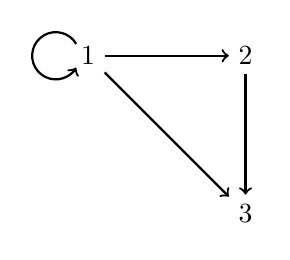
\begin{tikzpicture}
\node (atom1) at (0,2) {1};
\node (atom2) at (2,2) {2};
\node (atom3) at (2,0) {3};
\draw[->, thick] (atom1)--(atom2);
\draw[->, thick] (atom1)--(atom3);
\draw[->, thick] (atom1)+(-0.15,0.15) arc (-330:-30:.3); 
\draw[->, thick] (atom2) -- (atom3);
\end{tikzpicture}
\end{center}
De acordo com as convenções ali apresentadas, o domínio dessa interpretação são os três primeiros números inteiros positivos, e a extensão de  `$\atom{R}{x,y}$' é dada pelas setas do diagrama.
Ou seja, `$\atom{R}{x,y}$' é verdadeira para $\langle x, y \rangle$ apenas caso haja uma seta partindo  de \textbf{x} e chegando em \textbf{y} em nosso diagrama.
Aqui estão algumas sentenças verdadeiras nesta interpretação:
	\begin{ebullet}
		\item $\forall x \exists y\, \atom{R}{y,x}$ 
		\item $\exists x \forall y\, \atom{R}{x,y}$ \hfill  {\footnotesize 1 é uma testemunha}
		\item $\exists x \forall y (\atom{R}{y,x} \eiff x = y)$ \hfill {\footnotesize 1 é uma testemunha}
		\item $\exists x \exists y \exists z ((\enot y = z \eand \atom{R}{x,y}) \eand \atom{R}{z,x})$ \hfill {\footnotesize 2 é uma testemunha}
		\item $\exists x \forall y\, \enot \atom{R}{x,y}$ \hfill {\footnotesize 3 é uma testemunha}
		\item $\exists x (\exists y\, \atom{R}{y,x} \eand \enot \exists y\, \atom{R}{x,y})$ \hfill {\footnotesize 3 é uma testemunha}
	\end{ebullet}
Examine-as com cuidado e certifique-se de entender por que elas são todas verdadeiras na interpretação descrita pelo diagrama acima.\footnote{
	À direita de cada sentença existencial está indicada uma \textit{testemunha}, um elemento do domínio que satisfaz a fórmula existencialmente quantificada.
	Ou seja, cada uma destas sentenças é do tipo $\exists x \atom{\meta{A}}{x}$ e cada testemunha indicada corresponde a um indivíduo $\meta{c}$ do domínio para o qual $\atom{\meta{A}}{\meta{c}}$ é verdadeira na interpretação.}	
	
Isso também mostra que essas seis sentenças são compatíveis.
Podemos, então, usar esta observação para gerar argumentos \emph{inválidos}, tais como:
\begin{earg}
	\item[] $\forall x \exists y\, \atom{R}{y,x}$
	\item[] $\exists x \forall y\, \atom{R}{x,y}$
	\item[\therefore] $\forall x \exists y\, \atom{R}{x,y}$\footnote{
		Esta sentença não está entre os exemplos acima, porque ela é falsa em nossa interpretação.
		Para perceber isso basta notar que o indivíduo 3 é uma \textit{contratestemunha}, ou seja, é um elemento do domínio que não satisfaz a fórmula quantificada universalmente.}
\end{earg}
e
\begin{earg}
	\item[] $\exists x \forall y\, \atom{R}{x,y}$
	\item[] $\exists x \forall y \enot \atom{R}{x,y}$
	\item[\therefore] $\enot \exists x \exists y \exists z (\enot y = z \eand (\atom{R}{x,y} \eand \atom{R}{z,x}))$
\end{earg}

	\factoidbox{
	Ao apresentar uma interpretação em que  $\meta{A}_1$, $\meta{A}_2$, \dots, $\meta{A}_n$ são todas verdadeiras e onde $\meta{C}$ é falsa, nós mostramos que:
	\begin{ebullet}
		\item o argumento $\meta{A}_1, \meta{A}_2, \ldots, \meta{A}_n \therefore \meta{C}$ é inválido.
		\item $\meta{A}_1$, $\meta{A}_2$, \dots, $\meta{A}_n$ não sustentam $\meta{C}$.
		\item $\meta{A}_1$, $\meta{A}_2$, \dots, $\meta{A}_n$, $\enot \meta{C}$ são compatíveis.
	\end{ebullet}}
Uma interpretação que refuta uma proposta, ou seja, que mostra que um argumento \emph{não} é válido, ou que uma sentença \emph{não} é uma validade (logicamente necessária), ou que um conjunto de sentenças \emph{não} sustenta uma outra sentença, é chamada de \emph{contrainterpretação} ou \emph{contramodelo}.



\practiceproblems

\solutions
\problempart
\label{pr.Contingent}
Mostre que cada uma das seguintes sete sentenças não é nem uma validade (necessidade lógica) nem uma contradição.
\begin{earg}
\item \leftsolutions\ $\atom{D}{a}  \eand \atom{D}{b}$
\item \leftsolutions\ $\exists x\, \atom{T}{x,h}$
\item \leftsolutions\ $\atom{P}{m}  \eand \enot\forall x\, \atom{P}{x}$
\item $\forall z \atom{J}{z} \eiff \exists y\, \atom{J}{y}$
\item $\forall x (\atom{W}{x,m,n} \eor \exists y\atom{L}{x,y})$
\item $\exists x (\atom{G}{x} \eif \forall y\, \atom{M}{y})$
\item $\exists x (x = h \eand x = i)$
\end{earg}

\solutions
\problempart
\label{pr.NotEquiv}
Mostre que as sentenças de cada um dos nove pares seguintes não são logicamente equivalentes.
\begin{earg}
\item $\atom{J}{a} $,  $\atom{K}{a}$
\item $\exists x\, \atom{J}{x}$,  $\atom{J}{m}$
\item $\forall x\, \atom{R}{x,x}$, $\exists x\, \atom{R}{x,x}$
\item $\exists x\, \atom{P}{x} \eif \atom{Q}{c}$, $\exists x (\atom{P}{x} \eif \atom{Q}{c})$
\item $\forall x(\atom{P}{x} \eif \enot \atom{Q}{x})$, $\exists x(\atom{P}{x} \eand \enot \atom{Q}{x})$
\item $\exists x(\atom{P}{x} \eand \atom{Q}{x})$, $\exists x(\atom{P}{x} \eif \atom{Q}{x})$
\item $\forall x(\atom{P}{x}\eif \atom{Q}{x})$, $\forall x(\atom{P}{x} \eand \atom{Q}{x})$
\item $\forall x\exists y\, \atom{R}{x,y}$, $\exists x\forall y\, \atom{R}{x,y}$
\item $\forall x\exists y\, \atom{R}{x,y}$, $\forall x\exists y\, \atom{R}{y,x}$
\end{earg}

\problempart
Mostre que as sentenças de cada um dos treze grupos abaixo são compatíveis.
\begin{earg}
\item  $\atom{M}{a}, \enot \atom{N}{a}, \atom{P}{a}, \enot \atom{Q}{a}$
\item $\atom{L}{e,e}, \atom{L}{e,g}, \enot \atom{L}{g,e}, \enot \atom{L}{g,g}$
\item $\enot (\atom{M}{a} \eand \exists x\, \atom{A}{x}), \atom{M}{a} \eor \atom{F}{a}, \forall x(\atom{F}{x} \eif \atom{A}{x})$
\item $\atom{M}{a} \eor \atom{M}{b}, \atom{M}{a} \eif \forall x \enot \atom{M}{x}$
\item $\forall y\, \atom{G}{y}, \forall x (\atom{G}{x} \eif \atom{H}{x}), \exists y \enot \atom{I}{y}$
\item $\exists x(\atom{B}{x} \eor \atom{A}{x}), \forall x \enot \atom{C}{x}, \forall x\bigl[(\atom{A}{x} \eand \atom{B}{x}) \eif \atom{C}{x}\bigr]$
\item $\exists x\, \atom{X}{x}, \exists x\, \atom{Y}{x}, \forall x(\atom{X}{x} \eiff \enot \atom{Y}{x})$
\item $\forall x(\atom{P}{x} \eor \atom{Q}{x}), \exists x\enot(\atom{Q}{x} \eand \atom{P}{x})$
\item $\exists z(\atom{N}{z} \eand \atom{O}{z,z}), \forall x\forall y(\atom{O}{x,y} \eif \atom{O}{y,x})$
\item $\enot \exists x \forall y\, \atom{R}{x,y}, \forall x \exists y\, \atom{R}{x,y}$
\item $\enot \atom{R}{a,a}$, $\forall x (x=a \eor \atom{R}{x,a})$
\item $\forall x\forall y\forall z[(x=y \eor y=z )\eor x=z]$, $\exists x\exists y\ \enot x= y$
\item $\exists x\exists y((\atom{Z}{x} \eand \atom{Z}{y} )\eand x=y)$, $\enot \atom{Z}{d}$, $d=e$
\end{earg}

\problempart
Mostre que cada um dos dez argumentos abaixo é inválido.
\begin{earg}
\item $\forall x(\atom{A}{x} \eif \atom{B}{x}) \therefore \exists x\, \atom{B}{x}$
\item $\forall x(\atom{R}{x} \eif \atom{D}{x}), \forall x(\atom{R}{x} \eif \atom{F}{x}) \therefore \exists x(\atom{D}{x} \eand \atom{F}{x})$
\item $\exists x(\atom{P}{x}\eif \atom{Q}{x}) \therefore \exists x\, \atom{P}{x}$
\item $\atom{N}{a} \eand \atom{N}{b} \eand \atom{N}{c} \therefore \forall x\, \atom{N}{x}$
\item $\atom{R}{d,e}, \exists x\, \atom{R}{x,d} \therefore \atom{R}{e,d}$
\item $\exists x(\atom{E}{x} \eand \atom{F}{x}), \exists x\, \atom{F}{x} \eif \exists x\, \atom{G}{x} \therefore \exists x(\atom{E}{x} \eand \atom{G}{x})$
\item $\forall x\, \atom{O}{x,c}, \forall x\, \atom{O}{c,x} \therefore \forall x\, \atom{O}{x,x}$
\item $\exists x(\atom{J}{x} \eand \atom{K}{x}), \exists x \enot \atom{K}{x}, \exists x \enot \atom{J}{x} \therefore \exists x(\enot \atom{J}{x} \eand \enot \atom{K}{x})$
\item $\atom{L}{a}b \eif \forall x\, \atom{L}{x,b}, \exists x\, \atom{L}{x,b} \therefore \atom{L}{b,b}$
\item $\forall x(\atom{D}{x} \eif \exists y\, \atom{T}{y,x}) \therefore \exists y \exists z\ \enot y= z$
\end{earg}


\chapter[Infinitas interpretações]{Raciocinando sobre uma infinidade de interpretações}\label{s:InfinitInterpret}

\section{Validades e contradições}
Para mostrar que uma sentença não é uma validade basta apresentarmos uma única interpretação na qual a sentença é falsa.
Mas para mostrar que uma sentença é uma validade, não é suficiente propor dez, cem, nem mesmo mil interpretações nas quais a sentença é verdadeira.
Uma sentença é uma validade apenas se for verdadeira em \emph{todas} as interpretações; e há infinitas delas.
Precisamos ser capazes de raciocinar sobre todas elas, e não conseguiremos fazer isso lidando com elas uma de cada vez!

Raciocinar sobre todas as infinitas interpetações pode soar uma tarefa impossível.
Mas não é.
Algumas vezes nem  é tão complicado.
Veja como podemos mostar que a sentença \mbox{`$\atom{R}{a,a}\eor\enot \atom{R}{a,a}$'} é uma validade:
	\begin{quote}
		\label{allmodels1}
		Qualquer interpretação relevante (ou seja que leve em consideração a relação `$R$' e o nome `$a$') atribui um valor de verdade à sentença `$\atom{R}{a,a}$', que será verdadeira ou falsa.
		Então, se pensarmos na totalidade das interpretações relevantes, podemos dividir esta totalidade em dos grupos, o grupo (1), constituído pelas interpretações em que `$\atom{R}{a,a}$' é verdadeira, e o grupo (2), com as interpretações em que  `$\atom{R}{a,a}$' é falsa.
		`$\atom{R}{a,a}\eor\enot \atom{R}{a,a}$' será verdadeira em todas as interpretações do grupo (1), já que em todas elas `$\atom{R}{a,a}$' é verdadeira.
		Nas interpretações do grupo (2), como  `$\atom{R}{a,a}$' é falsa em todas elas, sabemos que `$\enot \atom{R}{a,a}$' é verdadeira em todas elas, e por isso, `$\atom{R}{a,a}\eor\enot \atom{R}{a,a}$' também é verdadeira em todas as interpretações do grupo(2).
		Como a sentença `$\atom{R}{a,a}\eor\enot \atom{R}{a,a}$' é verdadeira em todas as interpretações do grupo (1) e do grupo (2), e qualquer interpretação está em um destes dois grupos, então `$\atom{R}{a,a}\eor\enot \atom{R}{a,a}$' é verdadeira em todas as interpretações e é, por isso, uma validade.
		%Como os grupos (1) e (2) esgotam todas as interpretações e a sentença `$\atom{R}{a,a}\eor\enot \atom{R}{a,a}$' é verdadeira em todas as interpretações destes dois grupos, então ela é verdadeira em todas as interpretações, e por isso é uma validade.
	\end{quote}
Esta explicação é, ela própria, um argumento válido, e sua conclusão é verdadeira. Mas esta explicação não é um argumento na LPO, é um argumento em português \emph{sobre} a LPO; ou seja, é um argumento em nossa metalinguagem.

Uma outra característica deste nosso argumento metalinguístico é que como a sentença em questão não contém quantificadores, não precisamos pensar em como interpretar `$a$' e `$R$'; dissemos apenas que qualquer que seja a interpretação,  `$\atom{R}{a,a}$' será verdadeira ou falsa.
Poderíamos ter argumentado de modo similar a respeito de sentenças da LVF.

Eis aqui um outro exemplo de raciocínio sobre todas as interpretações.
Considere a sentença `$\forall x(\atom{R}{x,x}\eor\enot \atom{R}{x,x})$'.
Novamente, esta sentença parece uma validade óbvia, mas explicar precisamente por quê, é um grande desafio.
Não podemos dizer simplesmente que `$\atom{R}{x,x} \eor\enot \atom{R}{x,x}$' é verdadeira em todas as interpretações, uma vez que `$\atom{R}{x,x} \eor\enot \atom{R}{x,x}$' não é nem mesmo uma \emph{sentença} da LPO (lembre-se de que `$x$' é uma variável, não um nome).
Temos, então, que ser um pouco mais espertos.
	\begin{quote}
		Considere uma interpretação arbitrária.
		`$\forall x(\atom{R}{x,x}\eor \enot\atom{R}{x,x})$' será verdadeira nessa interpretação se e somente se `$\atom{R}{x,x}\eor\enot\atom{R}{x,x}$' for satisfeita por todos os objetos do domínio.
		Considere algum membro arbitrário do domínio, que, por conveniência, chamaremos de Zé.
		Ou Zé satisfaz `$\atom{R}{x,x}$', ou não.
		Se ele satisfaz `$\atom{R}{x,x}$', então Zé também satisfaz `$\atom{R}{x,x}\eor\enot\atom{R}{x,x}$'.
		Se Zé não satisfaz `$\atom{R}{x,x}$', ele certamente satisfaz `$\enot\atom{R}{x,x}$' e, portanto, também satisfaz `$\atom{R}{x,x}\eor\enot\atom{R}{x,x}$'.\footnote{
			Usamos aqui o fato de que as condições de verdade para os conectivos também se aplicam à satisfação:
		$a$ satisfaz $\meta{A}(\meta{x}) \lor \meta{B}(\meta{x})$ se e somente se $a$ satisfaz $\meta{A}(\meta{x})$ ou $\meta{B}(\meta{x})$, etc.
		}
		Então, em qualquer dos casos Zé satisfaz `$\atom{R}{x,x} \eor\enot \atom{R}{x,x}$'.
		Como não levamos em conta nenhuma característica específica de Zé---poderíamos ter escolhido qualquer outro indivíduo do domínio---o que dissemos sobre Zé vale também para qualquer outro objeto do domínio.
		Então, todo objeto no domínio satisfaz `$\atom{R}{x,x}\eor\enot\atom{R}{x,x}$'.
		Portanto, `$\forall x (\atom{R}{x,x} \eor\enot \atom{R}{x,x})$' é verdadeira em nossa interpretação.
		Mas também escolhemos nossa interpretação arbitrariamente, portanto `$\forall x (\atom{R}{x,x} \eor\enot \atom{R}{x,x})$' é verdadeira em todas as interpretações.
		É, por isso, uma validade.
	\end{quote}
Esta é uma explicação bastante longa e tediosa, mas não há alternativas aqui. Para mostrar que uma sentença é uma validade precisamos raciocinar sobre \emph{todas} as interpretações.
Considerando que a quantidade delas é infinita, até que nosso raciocínio não foi tão longo assim!


\section{Outros casos}
Há outros casos que também exigem que raciocinemos sobre todas as interpretações. Devemos fazê-lo se quisermos mostrar:
	\begin{ebullet}
	\item que uma sentença é uma contradição; pois isso requer que ela seja falsa em \emph{todas} as interpretações.
	\item que duas sentenças são logicamente equivalentes; pois isso requer que elas tenham o mesmo valor de verdade em \emph{todas} as interpretações.
	\item que algumas sentenças são incompatíveis; pois isso requer que não haja interpretação na qual todas essas sentenças sejam verdadeiras; ou seja, que, em \emph{toda} interpretação, pelo menos uma dessas sentenças seja falsa.
	\item que um argumento é válido; pois isso requer que a conclusão seja verdadeira em \emph{toda} interpretação em que as premissas são verdadeiras.
	\item que algumas sentenças sustentam alguma outra; pois isso também requer que a sentença sustentada seja verdadeira em \emph{toda} interpretação na qual as sentenças que a sustentam são verdadeiras.
	\end{ebullet}
O problema é que, com as ferramentas que temos no momento, raciocinar sobre todas as interpretações é um sério desafio! Vamos ver apenas mais um exemplo. Aqui está um argumento que é obviamente válido:
	$$\forall x(\atom{H}{x} \eand \atom{J}{x}) \ \therefore \ \forall x\, \atom{H}{x}$$
Afinal de contas, se tudo é $H$ e $J$, então tudo é $H$.
Mas só conseguimos mostrar que este argumento é válido se mostrarmos o que deve ser verdadeiro em todas as interpretações nas quais a premissa é verdadeira.
Para mostrar isso temos que raciocinar da seguinte maneira:
	\begin{quote}
		Considere uma interpretação arbitrária na qual a premissa `$\forall x(\atom{H}{x} \eand \atom{J}{x})$' seja verdadeira.
		Segue-se que `$\atom{H}{x} \eand \atom{J}{x}$' é satisfeita por todos os objetos nesta interpretação.
		Então `$\atom{H}{x}$' também será satisfeita por todos os objetos.\footnote{
			Aqui, novamente, fazemos uso do fato de que qualquer objeto que satisfaça $\meta{A}(\meta{x}) \land \meta{B}(\meta{x})$ deve satisfazer a $\meta{A}(\meta{x})$ e $\meta{B}(\meta{x})$.
		}
		Logo, `$\forall x\, \atom{H}{x}$' deve ser verdadeira nesta interpretação.
		Como a única coisa que assumimos sobre a interpretação é que nela `$\forall x(\atom{H}{x} \eand \atom{J}{x})$' é verdadeira, então, a mesma conclusão deve valer para qualquer outra interpretação que satisfaça a mesma condição.
		Ou seja, qualquer interpretação na qual `$\forall x(\atom{H}{x} \eand \atom{J}{x})$' é verdadeira é tal que `$\forall x\, \atom{H}{x}$' também é verdadeira.
		Por isso o argumento é válido!
\end{quote}
Veja que mesmo para um argumento simples como esse, o raciocínio que demonstra sua validade é um pouco complicado. Para argumentos mais longos e complexos a demonstração de sua validade pode ser extremamente torturante.

A tabela a seguir indica, para todos os conceitos semânticos que vimos, se as demonstrações de que eles se aplicam ou não se aplicam exigem apenas \textbf{uma} interpretação ou se é necessário raciocinarmos sobre \textbf{todas} as interpretações.

\begin{center} %\small
\begin{tabular}{l l l}
\cline{1-3}
\textbf{Teste} & \textbf{Sim} & \textbf{Não}\\
 \hline
\cline{1-3}
a sentença é uma validade? & todas & uma \\
a sentença é uma contradição? &  todas  & uma \\
as sentenças são equivalentes? & todas & uma \\
as sentenças são compatíveis? & uma & todas \\
O argumento é válido? & todas & uma \\
As premissas sustentam a conclusão? & todas & uma \\
\cline{1-3}
\end{tabular}
\end{center}
\label{table.ModelOrArgument}



%\begin{center}\small
%\begin{tabular}{l l l}
%\cline{2-3}
% & \textbf{Sim} & \textbf{Não}\\
 %\hline
%\cline{2-3}
%necessidade? & todas as interpretações & uma interpretação\\
%contradição? &  todas as interpretações  & uma interpretação\\
%equivalência? & todas as interpretações & uma interpretação\\
%satisfação? & uma interpretação & todas as interpretações\\
%validade? & todas as interpretações & uma interpretação\\
%sustentação? & todas as interpretações & uma interpretação\\
%\end{tabular}
%\end{center}
%\label{table.ModelOrArgument}

Pode ser útil comparar esta tabela com a que apresentamos para a LVF no final do Capítulo \ref{s:PartialTruthTable}, p.\,\pageref{t:TruthTable}.
A principal diferença está no fato de que a LVF diz respeito a tabelas de verdade, enquanto a LPO lida com interpretações.
Essa diferença, no entanto, é profundamente importante, uma vez que as tabelas de verdade têm sempre uma quantidade finita de linhas, de modo que uma tabela de verdade completa é um objeto relativamente tratável.
Por outro lado, sempre existem infinitas interpretações diferentes para cada sentença, de modo que o raciocínio sobre todas as interpretações pode ser um assunto profundamente complicado.
